
\documentclass[twocolumn]{article}
\usepackage{mathpazo}
\usepackage{microtype}
\usepackage{times}
\usepackage{titlesec} % 1
\usepackage[colorlinks = true,
            linkcolor = blue,
            urlcolor  = blue,
            citecolor = blue,
            anchorcolor = blue]{hyperref}
%\usepackage{sectsty} % "제 1 절" ...

 %%%%%%%%%%%%%%%%%%%%%%%%%%%%%%%%%%%%%%%%%%%%%%%%%%%%%%%%%%%%%%%%%%%%%%%%%%%%%
 %                              My Commands
\newcommand{\bi}{\begin{itemize}}
\newcommand{\ei}{\end{itemize}}
\newcommand{\be}{\begin{enumerate}}
\newcommand{\ee}{\end{enumerate}}
\newcommand{\ii}{\item}
\newtheorem{Def}{Definition}
\newtheorem{Lem}{Lemma}
\usepackage{algorithm}
\usepackage{algorithmicx}
\usepackage{algpseudocode}

\usepackage{graphicx}
\graphicspath{%
        {converted_graphics/}
        {./images/}
}

\usepackage{color}
\usepackage{xcolor}
\usepackage{listings}
\usepackage{caption}
\DeclareCaptionFont{white}{\color{white}}
\DeclareCaptionFormat{listing}{\colorbox{gray}{\parbox{\textwidth}{#1#2#3}}}
\captionsetup[lstlisting]{format=listing,labelfont=white,textfont=white}
\usepackage{verbatimbox}

\usepackage[hangul,nonfrench,finemath]{kotex}
    
\setlength\textwidth{7in} 
\setlength\textheight{9.5in} 
\setlength\oddsidemargin{-0.25in} 
\setlength\topmargin{-0.25in} 
\setlength\headheight{0in} 
\setlength\headsep{0in} 
%\setlength\columnsep{5pt}
\sloppy 
 
\begin{document}

\title{
\vspace{-0.5in}\rule{\textwidth}{2pt}
\begin{tabular}{ll}\begin{minipage}{4.75in}\vspace{6px}
\noindent\large {\it KIWI Project}@Data Management Research Section\\
\vspace{-12px}\\
\noindent\LARGE ETRI\qquad  \large Technical Report 15ZS1410-TR-65
\end{minipage}&\begin{minipage}{2in}\vspace{6px}\small
218 Gajeong-ro, Yuseong-gu\\
Daejeon, 305-700, South Korea\\
http:/$\!$/www.etri.re.kr/\\
http:/$\!$/sungsoo.github.com/\quad 
\end{minipage}\end{tabular}
\rule{\textwidth}{2pt}\vspace{0.25in}
\LARGE \bf 국외 출장 보고서 \\
\large A Survey on GPU-Accelerated Data Management Technologies
}

\date{}

\author{
{\bf Sung-Soo Kim}\\
\it{sungsoo@etri.re.kr}
}

\maketitle

\begin{abstract}
현재까지 하둡과는 별개로 GPGPU기반 데이터관리 사례로는 하버드와 MIT에서 개발한 대규모 스트림데이터 처리/분석/가시화를 수행할 수 있는 시스템인 MapD \cite{mapd:2015}가 있지만, 대부분 GPGPU기반 하둡 연구들은 실험결과 제시수준이다.
GPGPU를 통해 하둡기반 빅 데이터 시스템의 성능을 높이기 위해서는 GPU상에서 다루어야 할 \textit{데이터 저장/압축모델}, \textit{처리 방식} 뿐만 아니라, \textit{질의 처리} 방식도 GPU에 최적화되어야 한다.
\end{abstract}

\section{본론}

\subsection{Keynote Presentation}
슈퍼컴퓨팅 변화에 대한 소프트웨어 변화전략, GPU 기반 클라우드 가속화 기술, e-Science를 위한 복합 e-Infrastructure, 유럽지역의 컴퓨팅 인프라 및 로드맵인  EGI-Engage등 4개 주제로 키노트 발표가 있었다. 본 절에서는 슈퍼컴퓨팅 변화에 대한 소프트웨어 변화전략과 GPU 기반 클라우드 가속화 기술에 대한 키노트 발표에 대해 기술한다.

\subsubsection{Architecture-aware Algorithms and Software for Peta and Exascale Computing}
\textbf{Speaker:} Jack Dongarra\\
University of Tennessee and Oak Ridge National Lab, Tennessee, USA; University of Manchester, U.K.

\noindent
\textbf{Contributions:} 본 키노트 발표에서는 지난 10년 동안 고성능 컴퓨팅 기술 변화에 대해 살펴보고, 주요 기술 동향에 따른 미래 예상되는 HPC 기술들에 대해 설명해 주었다. 그림 \ref{fig:hpc_20}은 지난 20년간 HPC 성능개발 변화 추이를 그래프이다. 현재 아이폰은 20년전 슈퍼컴퓨터의 성능과 동일함을 알 수 있다. 하지만, 발표자는 이러한 하드웨어 성능 개선속도에 비해 소프트웨어 변화가 더딘면이 있다고 지적했다.

\begin{figure}[htb]
        \centering
        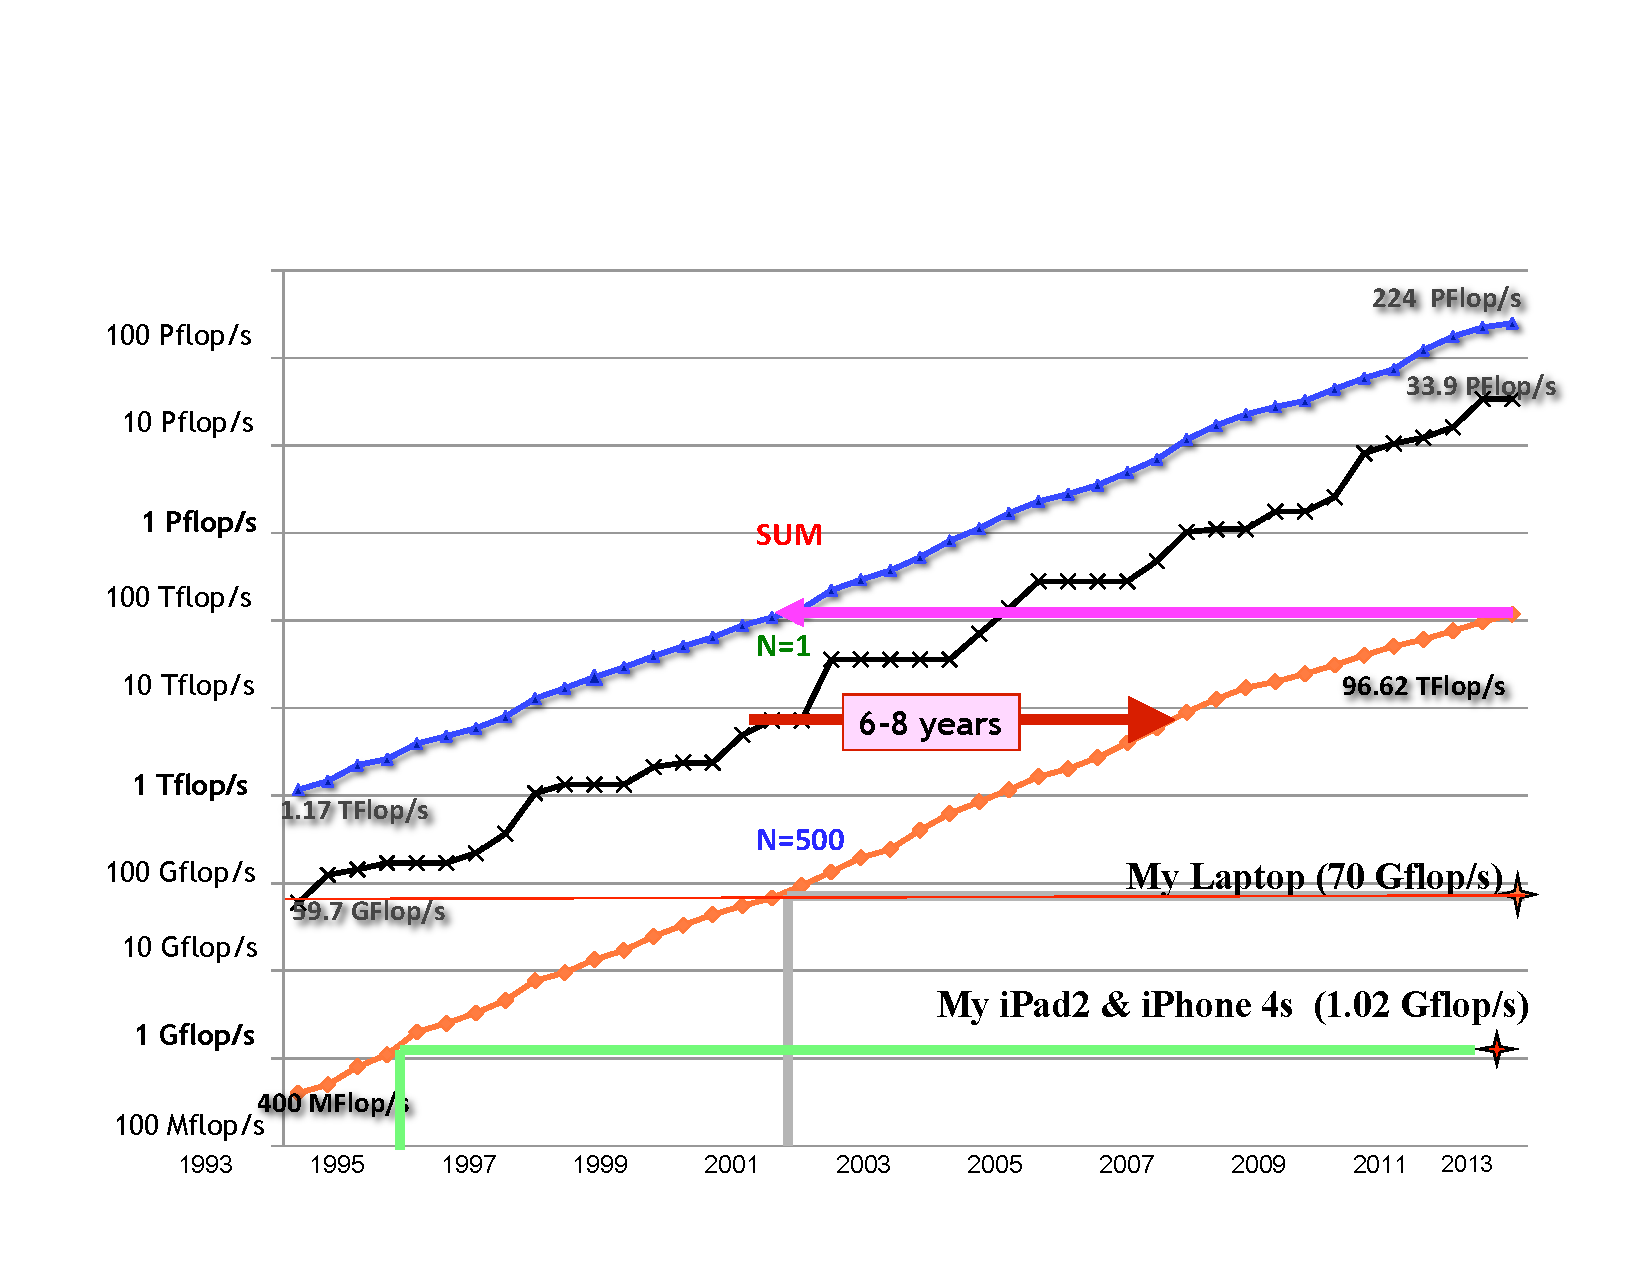
\includegraphics[width=0.48\textwidth]{hpc-20-years.pdf}
        \caption{Performance development of HPC over the last 20 years.}
        \label{fig:hpc_20}
\end{figure}
\noindent
\textbf{Why:}  지난 20년간 HPC 분야는 하드웨어 측면만을 지나치게 강조해서 연구개발 투자가 이루어져 왔다. HPC 기술 및 패러다임 변화는 우리가 개발하는 소프트웨어에 큰 영향을 미치기 때문에, HPC 기술이 어떻게 진화해 왔는지 그리고 앞으로 어떤 기술변화가 일어날 것인가 예측하는 것은 매우 중요하다. 현재 Top500의 99\% 시스템은 멀티코어 기반의 시스템이라고 한다. 따라서, 이러한 하드웨어 시스템 변화에 대응하는 소프트웨어 변화가 필요하다. 그림 \ref{fig:hpc_cores}는 슈퍼컴퓨터당 평균 코어수 변화 추이를 보여주고 있다.

\begin{figure}[htb]
        \centering
        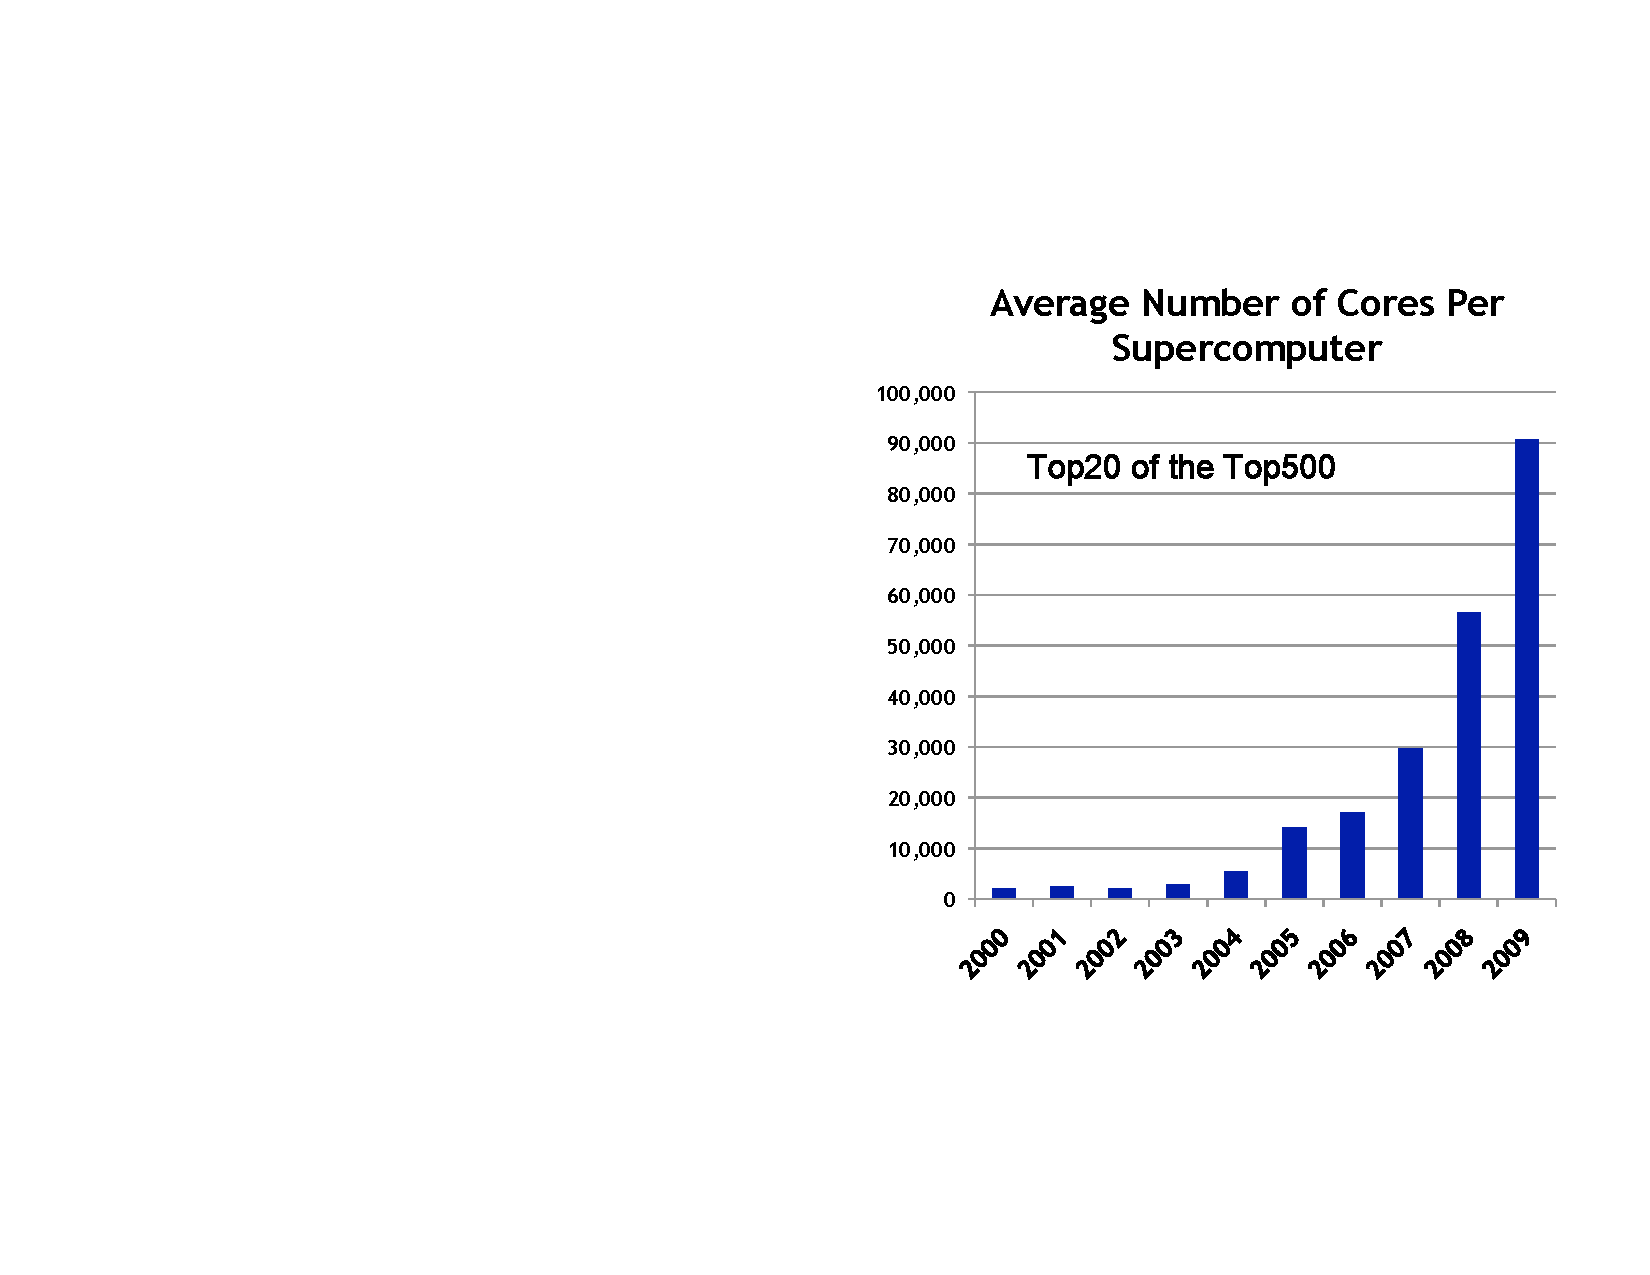
\includegraphics[width=0.48\textwidth]{hpc_cores.pdf}
        \caption{Average number of cores per supercomputer.}
        \label{fig:hpc_cores}
\end{figure}

\noindent
\textbf{How:}  소프트웨어 및 알고리즘 개발에 영향을 미칠 주요한 다섯가지 연구영역으로 나누어 기술변화를 예측하였다.
\bi
\ii 멀티코어 및 하이브리드 아키텍쳐에 맞게 소프트웨어 재설계 
\ii 자동 조정되는 응용 소프트웨어
\ii  성능을 위한 혼합 정밀도 활용하기
\ii 내고장성의 중요성
\ii 통신 회피 알고리즘
\ei

\noindent
\textbf{What:} Exascale computing으로 진화해 나가고 있는 HPC 하드웨어 및 소프트웨어 기술은 다음과 같다.
\bi
\ii Large-scale optics based interconnects
\ii Hardware and software based fault management
\ii Heterogeneous cores
\ii Another \textit{disruptive} technology
\bi
\ii Similar to what happened with \textit{cluster computing} and \textit{message passing}
\ei
\ei

\subsubsection{The Accelerated Cloud}
\textbf{Speaker:} Marc Hamilton\\
Vice President, Solutions Architecture and Engineering, NVIDIA, California, USA
\begin{figure}[htb]
        \centering
        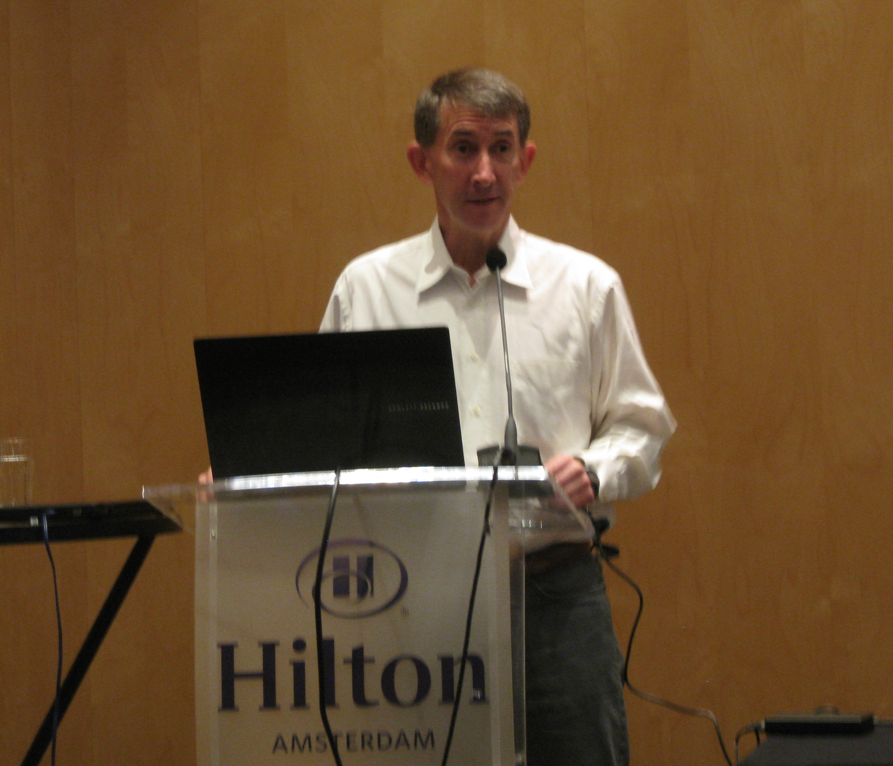
\includegraphics[width=0.45\textwidth]{marc.png}
        \caption{Marc Hamilton, NVIDIA}
        \label{fig:marc}
\end{figure}

\noindent
\textbf{Contributions:} 본 키노트 발표에서는 
지난 10년 동안 고성능 컴퓨팅 기술 변화에 대해 살펴보고, 주요 기술 동향에 따른 미래 예상되는 HPC 기술들에 대해 설명해 주었다. 
그림 \ref{fig:hpc_20}은 지난 20년간 HPC 성능개발 변화 추이를 그래프이다. 현재 아이폰은 20년전 슈퍼컴퓨터의 성능과 동일함을 알 수 있다. 하지만, 발표자는 이러한 하드웨어 성능 개선속도에 비해 소프트웨어 변화가 더딘면이 있다고 지적했다.


% Example Figure
%%%%%%%%%%%%%
%\begin{figure}[htb]
%        \centering
%        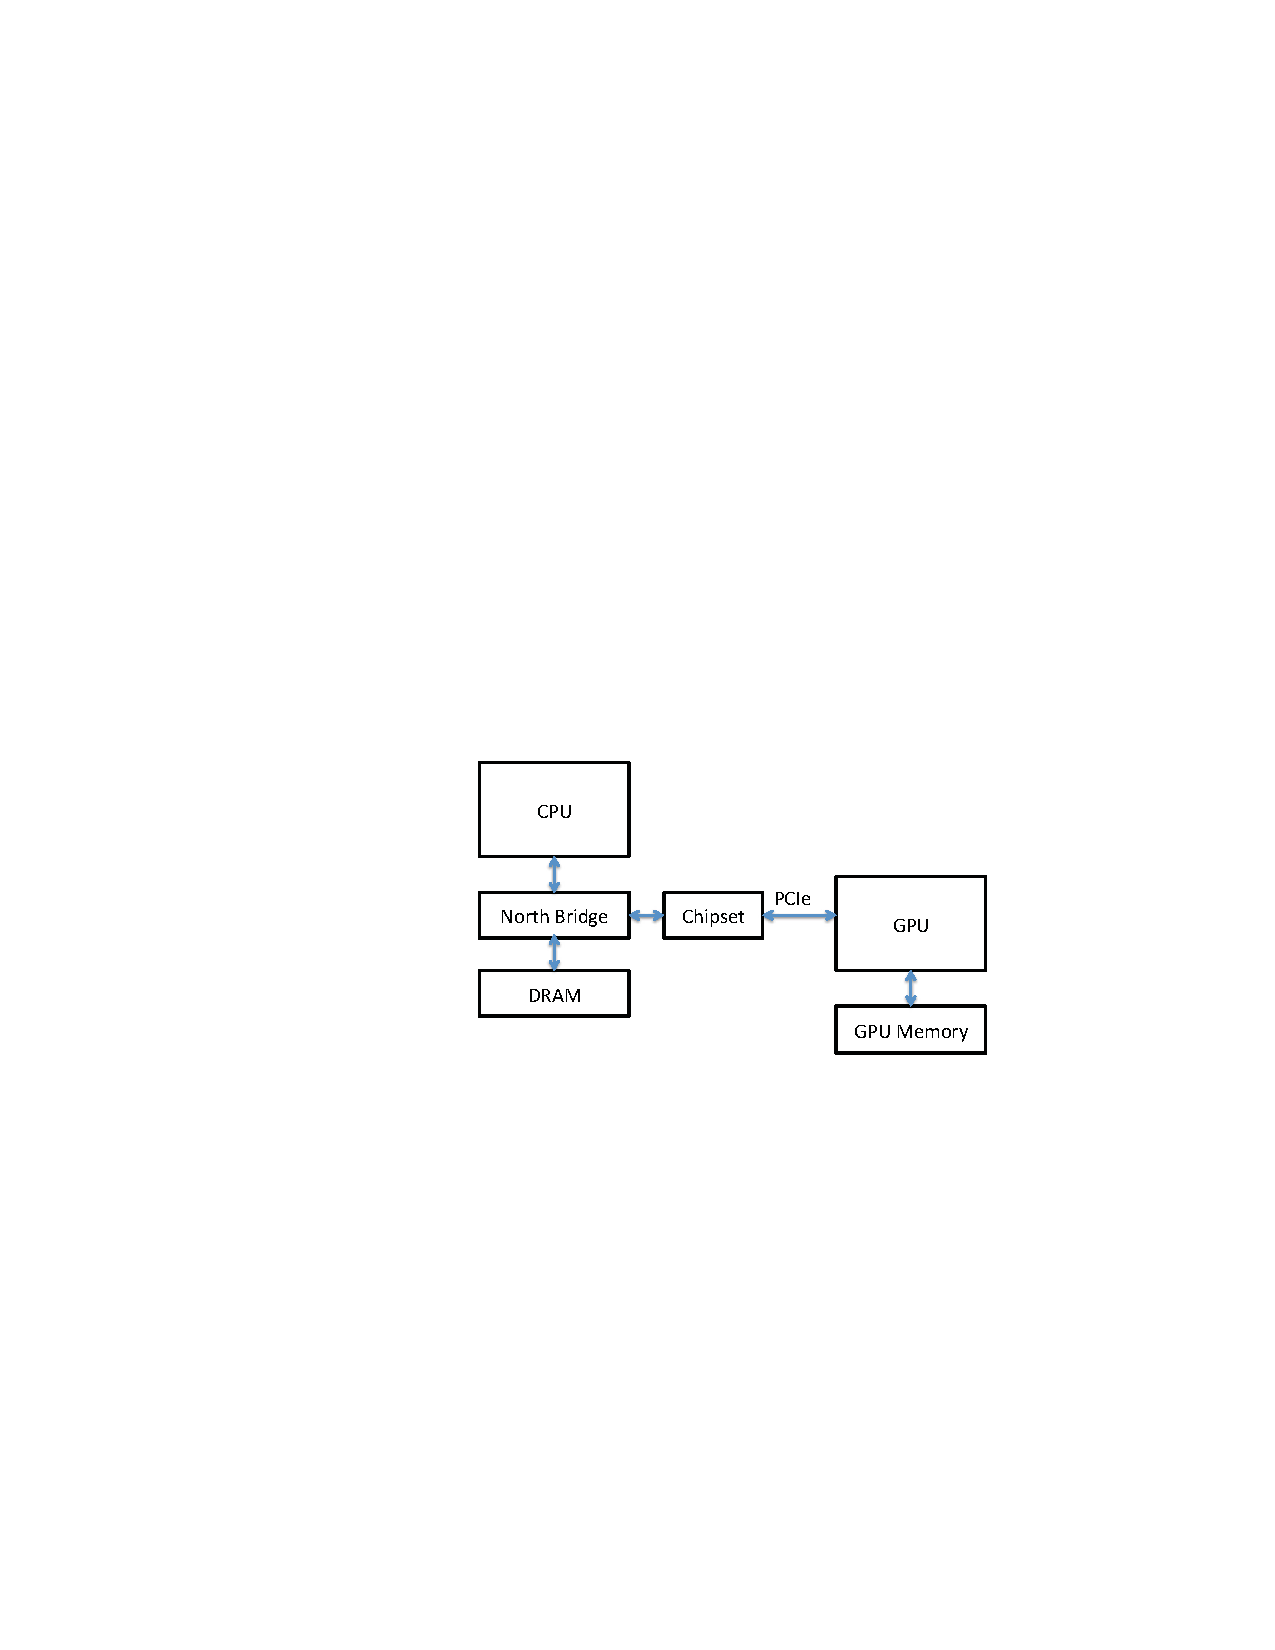
\includegraphics[width=0.48\textwidth]{system-overview.pdf}
%        \caption{A system overview with CPU and a discrete GPU.}
%        \label{fig:system_overview}
%\end{figure}

\begin{figure}[htb]
        \centering
        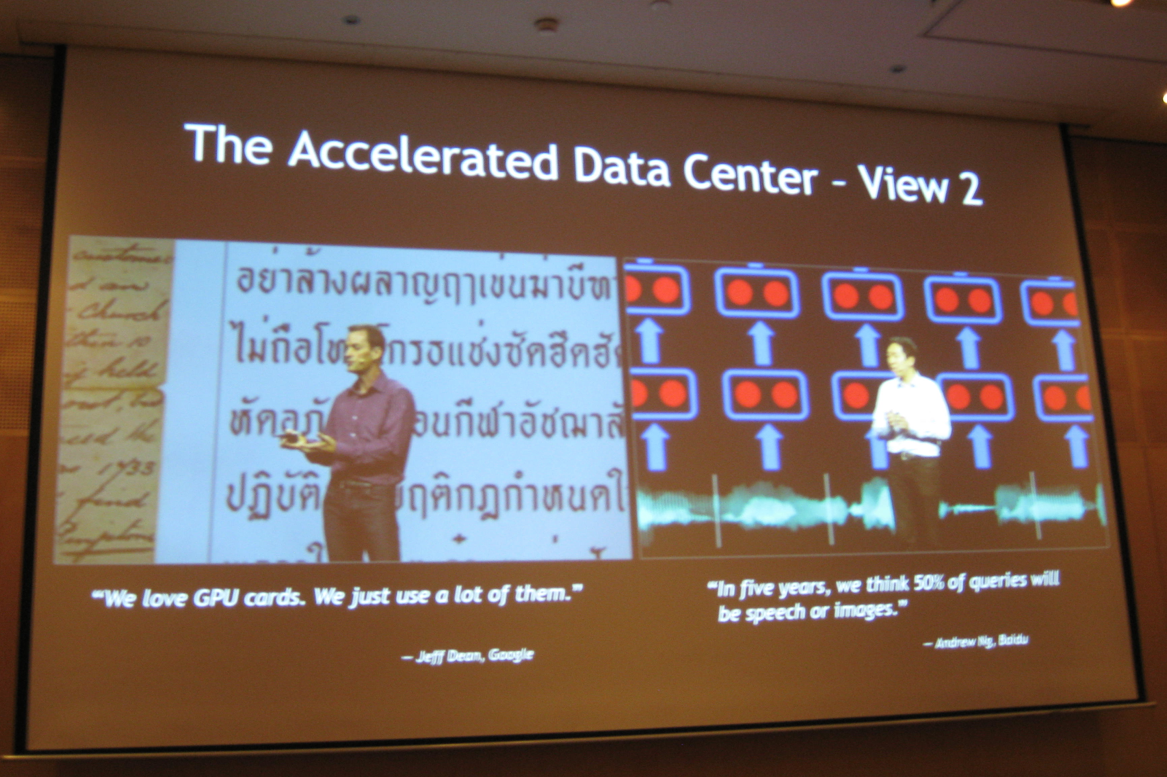
\includegraphics[width=0.48\textwidth]{marc-ppt.png}
        \caption{The Accelerated Data Center - View}
        \label{fig:marc-ppt}
\end{figure}

\bibliographystyle{abbrv}
\bibliography{sqlonhadoop}

\end{document}
